\documentclass[UTF8]{article}
\usepackage{CTEX}

\begin{document}
\section{UFL 博弈}\label{section:UFL}
在一个UFL博弈中,有一个双向网络图定义为 $G=(M,N,E)$, 其中 $M$ 为潜在工厂开设的集合,$N$ 为必须被服务顾客的集合,$E$ 为连接工厂和顾客所形成边的集合。每一个工厂潜在开设点 $i \in M$ 都有一个固定开启成本 $f_i$,并且每一条边 $(i,j) \in E$ 都有一个运输成本 $c_{ij}$。在UFL博弈中,顾客分享工厂开启和运输的成本,即在博弈中的参与者是顾客。我们在表中列出了在UFL中需要用到的记号。

\begin{table}[H]
\vspace{-2mm}
\tabcolsep=7pt
\small
\renewcommand\arraystretch{1.5}
\caption{\label{table:notationsUFL} Notation used in the UFL game}
\vglue5pt
\begin{tabular}[!h]{c c}
\hline
%\multicolumn{1}{c}{Symbol} &\multicolumn{1}{c}{Meaning}\\
%\cline{1-2}
\multicolumn{1}{c}{$M$} &\multicolumn{1}{l}{The set of potential facility sites, $M=\big\{1,2,...,m\big\}$.}\\
\multicolumn{1}{c}{$N$} &\multicolumn{1}{l}{The set of customer points as well as game players, $N=\big\{1,2,...,n\big\}$.}\\
\multicolumn{1}{c}{$c_{ij}$} &\multicolumn{1}{l}{Transportation cost from facility $i$ to customer $j$, $\forall i \in M, j \in N$.}\\
\multicolumn{1}{c}{$f_i$} &\multicolumn{1}{l}{Fixed opening cost of facility $i$, $\forall i \in M$.}\\
\multicolumn{1}{c}{$s$} &\multicolumn{1}{l}{Player coalition, $s \subseteq N$.}\\
\multicolumn{1}{c}{$\gamma^s$} &\multicolumn{1}{l}{Incidence vector $\big[ \gamma^{s}_1,\gamma^{s}_2,...,\gamma^{s}_{n}\big]^T$, where $\gamma^{s}_j=1$ if player $j$ is in coalition $s$ and $\gamma^{s}_j=0$ otherwise.}\\
\multicolumn{1}{c}{$v_i$} &\multicolumn{1}{l}{Decision variable, where $v_i=1$ if facility $i$ will be opened and $v_i=0$ otherwise, $\forall i \in M$.}\\
\multicolumn{1}{c}{$u_{ij}$} &\multicolumn{1}{l}{Decision variable, where $u_{ij}=1$ if customer $j$ will be served by facility $i$ and $u_{ij}=0$ otherwise,}\\
\multicolumn{1}{c}{} &\multicolumn{1}{l}{ $\forall i \in M$ and $j \in N$.}\\
\hline
\end{tabular}
\vspace{-3mm}
\end{table}

\begin{定义}\label{defi:ug}
UFL 博弈 $(N,c_{UFL})$ 的定义为,在集合 $N$ 中的顾客为参与者并且特征函数为 $c_{UFL}(s)$ 由如下的整数规划决定,

\begin{equation}\label{eqn:ugobj}
c_{UFL}(s) = \min_{v,u} \sum_{i \in M} f_iv_i + \sum_{i \in M} \sum_{j \in N} c_{ij}u_{ij}
\end{equation}
\begin{equation} \label{eqn:ugcon1}
s.t.~\sum_{i \in M} u_{ij} \geq \gamma_j^s, ~\forall j \in N,
\end{equation}
\begin{equation}\label{eqn:ugcon2}
u_{ij} - v_i \leq 0, ~\forall i \in M, j \in N,
\end{equation}
%\begin{equation}\label{eqn:ugcon3}
%u_{ij} \leq \gamma_j^s, ~\forall i \in M, j \in N
%\end{equation}
\begin{equation}\label{eqn:ugcon4}
v_i, u_{ij} \in \{0,1\}, ~\forall i \in M, j \in N.
\end{equation}
\end{definition}

在上述的整数规划中,目标函数 $(\ref{eqn:ugobj})$ 是为了最小化对于一个联盟 $s$ 中工厂开启和运输的总成本,限制条件 $(\ref{eqn:ugcon1})$ 需要在联盟 $s$ 中的每一位顾客被服务,而限制条件 $(\ref{eqn:ugcon2})$ 确保了只有一个开启的工厂可以服务顾客。

整数规划 (\ref{eqn:ugobj})-(\ref{eqn:ugcon4}) 是对于一个无容量限制的设施选址问题的常规表达式。基于定义, 我们可以看到UFL博弈 $(N,c_{UFL})$ 是一个OR博弈 $(V,c)$ 其中 $V=N$,$c = c_{UFL}$。特别地,在 $c$ 中的决策变量 $x$ 现在变为在$c_{UFL}$ 中的 $[v;u]$, 并且矩阵 $C$, $A$, $A'$, $B$, $B'$, $D$, $D'$ 的具体表达式也可以通过用矩阵写出 $c_{UFL}$ 而得到。 特别地,$D$ 和 $D'$ 现在都是 $\textbf{0}$,所以博弈 $(N,c_{UFL})$ 是次可加的。这一点对于我们接下来要研究的 ULCFL 博弈来说也是正确的。

\section{对于UFL博弈线性规划解的成本分配}
\cite{Kolen1983FacilityLocationGame} 和 \cite{Goemans2000FacilityLocationGames} 证明了,对于一个UFL博弈,最大稳定成本分配值与 $c_{UFL}(N)$ 的LP下界重合。为了做进一步的分析,我们给出了使用 LPB 算法来计算最优稳定成本分配的更多细节。

在 $c_{UFL}(s)$ 中,限制条件 $(\ref{eqn:ugcon1})$ 和 $(\ref{eqn:ugcon2})$ 已经是可分配的。通过加入可分配限制条件 $\{u_{ij} \geq 0:i \in M, j \in N\}$ 来松弛二元限制条件 (\ref{eqn:ugcon4}),我们可以得到一个对于大联盟最优解问题 $c_{UFL}(N)$ 的LP松弛如下:

\begin{equation*}\label{eqn:lpugobj}
c_{LP\_UFL}(N) = \min_{v,u} \sum_{i \in M} f_iv_i + \sum_{i \in M} \sum_{j \in N} c_{ij}u_{ij}
\end{equation*}
\begin{equation} \label{eqn:lpugcon1}
s.t.~\sum_{i \in M} u_{ij} \geq \gamma_j^N, ~\forall j \in N,
\end{equation}
\begin{equation}\label{eqn:lpugcon2}
v_i - u_{ij} \geq 0, ~\forall i \in M, j \in N,
\end{equation}
\begin{equation}\label{eqn:lpugcon3}
u_{ij} \geq 0, ~\forall i \in M, j \in N.
\end{equation}

我们有顺序地对限制条件$(\ref{eqn:lpugcon1})$, $(\ref{eqn:lpugcon2})$ 和 $(\ref{eqn:lpugcon3})$ 分别从 $1$ 到 $n$, $n+1$ 到 $n+mn$ 和 $n+mn+1$ 到 $n+2mn$ 进行标号。对于 $c_{LP\_UFL}(N)$,我们考虑它的对偶线性规划。让 $\mu_k$ 为$c_{LP\_UFL}(N)$ 的第 $k$ 个限制条件所对应的对偶变量, 并且 $\mu^*$ 为对偶式的最优解。
根据在附录中的行生成方法,我们有如下的引理:

\begin{lemma}\label{lemma:lpbcaufl}
对于一个 UFL 博弈,LPB 成本分配 $\alpha_{LP\_UFL}$ 由下式给出
\begin{equation*}
\alpha_{LP\_UFL}(j) = \mu_j^*, ~\forall j \in \big\{1,2,\ldots,n\big\},
\end{equation*}
是最优的, 同时总的共享成本为 $c_{LP\_UFL}(N)$.
\end{lemma}

我们记一种对于UFL博弈得到最优稳定成本分配的简单方式是直接解 $c_{LP\_UFL}(N)$ 并且通过计算限制条件的影子价格得到最优对偶变量。然而,解对偶线性规划有助于找到替代的最优解,因为在对偶LP有多个最优解的情况下,并不是所有的都对应于原始的影子价格。

\section{对于UFL博弈拉格朗日松弛解的成本分配}
接下来我们将演示如何应用LRB算法来获得UFL博弈的最优成本分配。我们将证明UFL博弈的子博弈2是次模的。我们还将通过计算实验表明,LRB算法所获得的该博弈的最优成本分配与LPB算法所获得的成本分配不同,从而为评价和比较提供更多的选择。

在 $c_{UFL}(s)$ 中,我们加入了一系列新的限制条件
\begin{equation}\label{eqn:UFLLRBC}
\big\{ u_{ij} \leq \gamma_j^s: ~\forall i \in M, j \in N\ \big\},
\end{equation}
然后引入限制条件 $\{ \sum_{i \in M} u_{ij} \geq \gamma_j^s:j \in N \}$ 到加入了非负拉格朗日乘子 $\sigma$ 的目标函数中,从而得到UFL的拉格朗日特征函数。

\begin{eqnarray*}\label{eqn:LRPGCF}
\begin{aligned}
\begin{split}
c_{LR\_UFL}(s;\sigma) = \min_{v,u} \sum_{i \in M} f_iv_i + &\sum_{i \in M} \sum_{j \in N} \big(c_{ij} - \sigma_{j}\big)u_{ij} + \sum_{j \in N} \sigma_j \gamma_j^s\\
s.t.~u_{ij} - v_i \leq 0,&~\forall i \in M, j \in N,\\
u_{ij} \leq \gamma_j^s,~\forall i& \in M, j \in N,\\
v_i,u_{ij} \in \{0,1\},~&\forall i \in M, j \in N.
\end{split}
\end{aligned}
\end{eqnarray*}

约束条件 $(\ref{eqn:UFLLRBC})$ 的增强是为了加强 $c_{UFL}(s)$ 的拉格朗日下界,这有可能因此得到更好的LRB成本分配。。
它禁止设置 $u_{ij'}=1$ 对于任何不在联盟s中的参与者,即使计算$c_{LR\_UFL}(s;\sigma)$时,系数 $c_{ij'}- \sigma_{j'}<0$。
很容易看出 $(\ref{eqn:UFLLRBC})$ 的增强只相当于在目标函数 $c_{LR\_UFL}(s;\sigma)$ 中替换术语 $\sum_{i \in M} \sum_{j \in N} \big(c_{ij} - \sigma_{j}\big)u_{ij}$ by $\sum_{i \in M} \sum_{j \in s} \big(c_{ij} - \sigma_{j}\big)u_{ij}$。

在算法 \ref{algolrb}下,一般的LRB成本分配算法对于任何 $s \in S$ 和非负拉格朗日乘子 $\sigma$, 我们可以分解 $c_{LR\_UFL}(s;\sigma)$ 为 $c_{LR1\_UFL}(\ \cdot \ ;\sigma)$ 和 $c_{LR2\_UFL}(\ \cdot \ ;\sigma)$ 使得 $c_{LR\_UFL}(s;\sigma) = c_{LR1\_UFL}(s;\sigma) + c_{LR2\_UFL}(s;\sigma)$, and define UFL sub-game 1 $\big(N,c_{LR1\_UFL}(\ \cdot \ ;\sigma)\big)$ and UFL sub-game 2  $\big(N,c_{LR2\_UFL}(\ \cdot \ ;\sigma)\big)$.

对于UFL的子博弈1,它的特征函数是

\begin{eqnarray}\label{eqn:UFLCFsub1}
\begin{aligned}
\begin{split}
c_{LR1\_UFL}(s;\sigma) = \sum_{j \in N} \sigma_j \gamma_j^s.
\end{split}
\end{aligned}
\end{eqnarray}

根据引理 $\ref{lemma:lr1core}$,最优稳定成本分配 $\alpha_{LR1\_UFL}^{\sigma}$ 位于由 $\alpha_{LR1\_UFL}^{\sigma}(j) = \sigma_j$ $j \in N$ 给出的博弈 $\big(N, c_{LR1\_UFL}(\ \cdot \ ;\sigma)\big)$ 的核中。

对于UFL的子博弈2,它的特征函数为
\begin{eqnarray}\label{eqn:UFLCFsub2}
\begin{aligned}
\begin{split}
c_{LR2\_UFL}(s;\sigma) = \min_{v,u} \sum_{i \in M} &f_iv_i + \sum_{i \in M} \sum_{j \in N} \big(c_{ij} - \sigma_{j}\big)u_{ij}\\
s.t.~u_{ij} - v_i \leq 0,&~\forall i \in M, j \in N,\\
u_{ij} \leq \gamma_j^s,~\forall i& \in M, j \in N,\\
 v_i,u_{ij}, \in \{0,1\},~&\forall i \in M, j \in N.
\end{split}
\end{aligned}
\end{eqnarray}
为了解 $c_{LR2\_UFL}(s:\sigma)$,我们可以将其分解为各种条件,并且得到一个闭式的由下式给出的最优目标函数值 $c_{LR2\_UFL}(s;\sigma) = \sum_{i=1}^m \min \big\{0,f_i+\sum_{j \in s} \min \{0,c_{ij}-\sigma_j\}\big\}$ 。

\begin{lemma}\label{lemma:UFLSubmodular}
UFL sub-game 2 $\big(N,c_{LR2\_UFL}(\ \cdot \ ;\sigma)\big)$ is submodular.
\end{lemma}
{\scshape Proof.}
Denote $a$ and $b$ as two players in $N$. To show the submodularity, we need to prove that, for any coalition $s \in N\setminus \big\{a,b\big\}$,
\begin{equation}\label{ll14}
c_{LR2\_UFL}(s \cup \{a\}; \sigma) - c_{LR\_UFL2}(s;\sigma) \geq c_{LR2\_UFL}(s \cup \big\{a,b\big\};\sigma) - c_{LR2\_UFL}(s \cup \{b\};\sigma).
\end{equation}

对于每一个 $i\in M$,令 $\Delta_i(s;\sigma) = \min \{0, f_i + \sum_{j \in s} \min \{0, c_{ij} - \sigma_j\} \}$。为了证明 (\ref{ll14}),足够证明

\begin{equation}\label{eqn:submodularufl}
\Delta_i(s;\sigma) + \Delta_i(s \cup \{a,b\};\sigma) \leq \Delta_i(s \cup \{a\};\sigma) + \Delta_i(s \cup \{b\};\sigma), ~\forall s \in N\setminus\big\{a,b\big\}. \end{equation}

令 $\rho(x)=\min\{0,x\}$,并且定义 $x_{\hat{s}}= f_i + \sum_{j \in \hat{s}} \min \{0, c_{ij} - \sigma_j\}$ for each $\hat{s}\in \{s,s\cup\{a\},s\cup\{b\},s\cup\{a,b\}\}$。
可以看出 $x_s+x_{s\cup\{a,b\}} = x_{s\cup \{a\}}+x_{s\cup\{b\}}$, 和 $x_{s\cup\{a,b\}}\leq \min\{x_{s\cup \{a\}},x_{s\cup\{b\}}\}\leq  \max\{x_{s\cup \{a\}},x_{s\cup\{b\}}\} \leq x_{s}$.
因此,既然 $\rho(x)$ 是一个关于 $x$ 的凹函数,我们有

\begin{eqnarray*}
  \rho(x_s) + \rho(x_{s\cup \{a,b\}}) \leq \rho(x_{s\cup\{a\}}) + \rho(x_{s\cup \{b\}}),
\end{eqnarray*}
从中我们可以直接得到 (\ref{eqn:submodularufl}),并且完成了引理的证明。
\hfill\Halmos

由于UFL子博弈2的次模性,我们能够很容易地计算它的核成本分配,记为 $\alpha_{LR2\_UFL}^{\sigma}$,通过子博弈章节中的贪心算法。在最优拉格朗日乘子 $\sigma^*$ 下,我们可以得到由 $\alpha_{LR\_UFL}^{\sigma^*} = \alpha_{LR1\_UFL}^{\sigma^*} + \alpha_{LR2\_UFL}^{\sigma^*}$ 给出的最优UFL的LRB成本分配。
既然UFL的子博弈1和子博弈2都有非空核,通过定理 \ref{thm:lagcostallocation1} 最优LRB成本分配值达到了拉格朗日下界 $c_{LR\_UFL}(N;\sigma^*)$,即不小于LP的下界 $c_{LP\_UFL}(N)$。

下面的定理说明了UFL LRB成本分配的最优性,并揭示了LRB和LPB成本分配的等价性。

\begin{theorem}\label{lemma:lpbequallrbufl}
For a UFL game, the LRB cost allocation $\alpha_{LR\_UFL}^{\sigma^*} = \sigma^* + \alpha_{LR2\_UFL}^{\sigma^*}$ is optimal. In addition, both the LRB cost allocation set and the LPB cost allocation set consist of all the optimal UFL cost allocations.
\end{theorem}
{\scshape Proof.}

对于UFL博弈,我们首先证明了LRB的成本分配是最优的。如前所述,最优LRB成本分配值达到拉格朗日下界 $c_{LR\_UFL}(N;\sigma^*)$,其不小于LP下界 $c_{LP\_UFL}(N)$。
我们知道对于UFL博弈的LP下界等于最大总共享成本 \citep{Kolen1983FacilityLocationGame,Goemans2000FacilityLocationGames}。因此,LRB成本分配一定是一个最优UFL成本分配,并且 $c_{LR\_UFL}(N;\sigma^*)=c_{LP\_UFL}(N)$。

然后,我们证明了LRB成本分配集和LPB成本分配集都包含所有的最优UFL成本分配。众所周知,LPB成本分配集由所有最佳UFL成本分配\citep{Goemans2000FacilityLocationGames}组成。这意味着每个LRB成本分配必须属于LPB成本分配集。因此,仍然需要证明,每个LPB成本分配都属于LRB成本分配集。

考虑到每一个LPB成本分配 $\alpha_{LP\_UFL}(j)=\mu^*_j$ for $j \in N$,这里 $\mu^*$ 和 一些 $\delta^*$ 构成一个最优解对于下面的关于 $c_{LP\_UFL}(N)$ 的对偶问题:

\begin{eqnarray*}
\begin{aligned}
\begin{split}\label{eqn:UFLLRdual1}
 \max_{\mu,\delta} \sum_{j \in N}&\mu_j\\
s.t.~\sum_{j \in N}\delta_{ij} = f_i&, ~\forall i \in M,\\
\mu_j - \delta_{ij} \leq c_{ij}, ~\forall i& \in M, j \in N,\\
 \mu_j \geq 0, \delta_{ij} \geq 0,~\forall &i \in M, j \in N.
\end{split}
\end{aligned}
\end{eqnarray*}

对每一个 $i\in M$, 可以看出 $f_i = \sum_{j\in N}\delta^*_{ij}$,并且 $\delta^*_{ij}\geq \max\{0,\mu^*_j-c_{ij}\}$ 对于 $j \in N$,这表明 $f_i \geq \sum_{j\in N}\max\{0,\mu^*_j-c_{ij}\}=-\sum_{j\in N}\min\{0,c_{ij}-\mu^*_j\}$。
因此,我们有
\begin{eqnarray}
  \min\{0,f_i + \sum_{j\in N}\min\{0,c_{ij}-\mu^*_j\}\} =0, \mbox{ for each $i\in M$.} \label{eqn:cost}
\end{eqnarray}
既然 $c_{LR2\_UFL}(N;\sigma)=\sum_{i=1}^{m}\min\{0,f_i+\sum_{j\in N}\min\{0,c_{ij}-\sigma_{j}\}\}$ 对于任何非负 $\sigma$ 成立,由 (\ref{eqn:cost}) 我们有 $c_{LR2\_UFL}(N;\mu^*) = 0$。
同时加上 $c_{LR1\_UFL}(N;\mu^*)=\sum_{j\in N}\mu^*_j$ 该式,表明 $c_{LR\_UFL}(N;\mu^*) = \sum_{j\in N}\mu^*_j = c_{LP\_UFL}(N)=c_{LR\_UFL}(N;\sigma^*)$。
因此 $\mu^*$ 是一个最优拉格朗日乘子。
由此产生的LRB成本分配如下:$\alpha^{\mu^*}_{LR\_UFL}(j) = \mu^*_j + \alpha^{\mu^*}_{LR2\_UFL}(j)$ for $j \in N$。
注意到对于每一个 $s\in S$,因为 $c_{LR2\_UFL}(s;\mu^*)\leq 0$ 和 $c_{LR2\_UFL}(s;\mu^*)\geq c_{LR2\_UFL}(N;\mu^*)=0$,我们有 $c_{LR2\_UFL}(s;\mu^*)=0$,这将得到 $\alpha^{\mu^*}_{LR2\_UFL}(j) = 0$ 对于所有 $j\in N$。
因此我们得到 $\alpha^{\mu^*}_{LR\_UFL} = \mu^*$,表明每一个LPB成本分配 $\mu^*$ 属于LRB成本分配集。这就完成了定理
\ref{lemma:lpbequallrbufl} 的证明。
\hfill\Halmos

\section{替代最优稳定成本分配}\label{section:uflcomputation}
对于一个UFL博弈,我们知道每一个最优成本分配对应于一个LPB解,它必须是对偶式 $c_{LP\_UFL}(N)$ 的所有基本最优解的凸组合。 然而,只应用一般的LP求解方法于 对偶式 $c_{LP\_UFL}(N)$ 是很难得到所有基本最优解的。

通过 \ref{lemma:lpbequallrbufl}, 我们知道LRB算法提供了对于UFL博弈的一种替代最优成本分配。所获得的LRB解有可能被排除在一般LP求解产生的LPB解之外。我们通过下面的例子来说明这一点。

\begin{figure}[H]
\centering
\vspace{-0.1em}
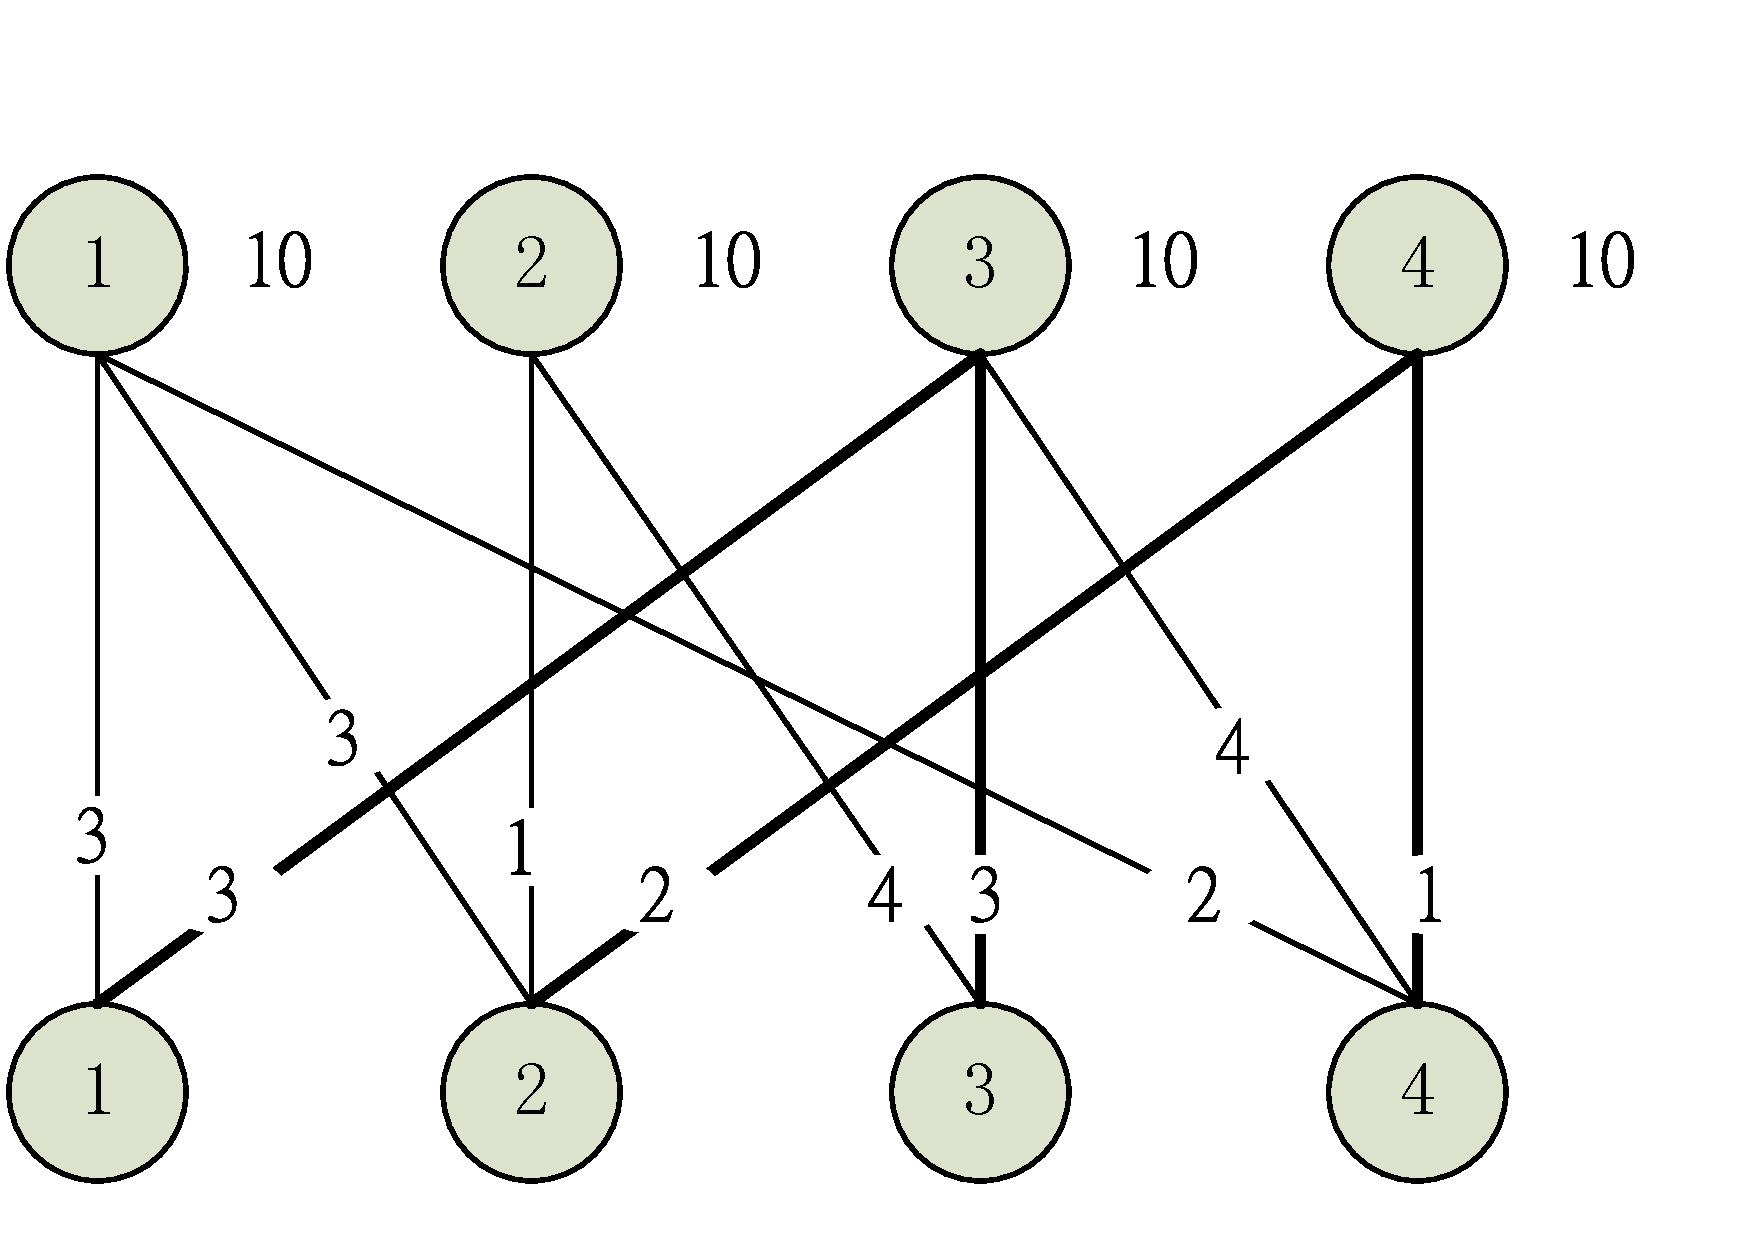
\includegraphics[width=0.5\textwidth]{figure-1.pdf}
\caption{\label{figure:exampleUFL}An example of a UFL game}
\vspace{-3mm}
\end{figure}

在图\ref{figure:exampleUFL}中所示的UFL博弈中,这里有四个设施和四个参与者。每一个设施有一个固定的启用成本10。在连接线上的数字代表从设施到参与者的运输成本。对于大联盟的一个最优解是开启设施3和4,并且画粗的连接线是最优路径。因此,大联盟所需要的成本是 10+10+3+3+2+1=29。

在这个例子中,我们使用了两种 LP 求解方法,单纯形法和内点法,分别在 MATLAB 发行版本 2011a上计算LPB分配。
表 \ref{table:UFLCA} 显示了在不同方法下的每一个参与者需要承担的成本。


\begin{table}[H]
\vspace{-2mm}
\centering
\tabcolsep=4pt
\small
\renewcommand\arraystretch{1.5}
\caption{\label{table:UFLCA} Optimal stable UFL cost allocations under different approaches}
\vglue5pt
\begin{tabular}[!h]{c c c c c c c c c c c c c}
\hline
\multicolumn{1}{c}{Method} &\multicolumn{1}{c}{} &\multicolumn{1}{c}{Player 1} &\multicolumn{1}{c}{} &\multicolumn{1}{c}{Player 2} &\multicolumn{1}{c}{} &\multicolumn{1}{c}{Player 3} &\multicolumn{1}{c}{} &\multicolumn{1}{c}{Player 4}	&\multicolumn{1}{c}{} &\multicolumn{1}{c}{Total Shared Cost}\\
\hline
LPB with Simplex	& &5.00	& &6.50	& &8.50	& &6.50	&	&26.5	&\\
LPB with Interior Point	& &6.58	& &6.50	& &8.50	& &4.92	&	&26.5	&\\
LRB	& &6.87	& &6.50	& &8.50	& &4.63	&	&26.5	&\\
\hline
\end{tabular}
\vspace{-3mm}
\end{table}

实例表明,LRB算法可以产生不同于一般LP方法的最优稳定成本分配。
LRB解超出了两个LPB解的凸组合范围。
这说明了LRB算法在提供替代成本分配方面的价值。

为了研究LRB算法在一般设置下的能力,我们测试了由 \cite{Benchmark} 开发的30个无容量限制的设施位置基准实例,所有实例均有 $ M=N=100$。我们在一台Windows7 个人电脑上进行了所有的计算实验,该电脑的CPU型号为英特尔酷睿i7-2600,主频3.4GHz和内存为16G。所有算法均在Matlab 2011a版本中实现。
在30个实例中,有22个实例的LRB解超出了两个LPB解的凸组合范围。
同样,这显示了LRB算法在计算上寻找替代最优稳定成本分配方面的价值,即使在LPB成本分配显示为最优的情况下也是如此。
